\subsection{\Large Progettazione Concettuale}

\newpage

\subsubsection{\Large Class Diagram non ristrutturato}

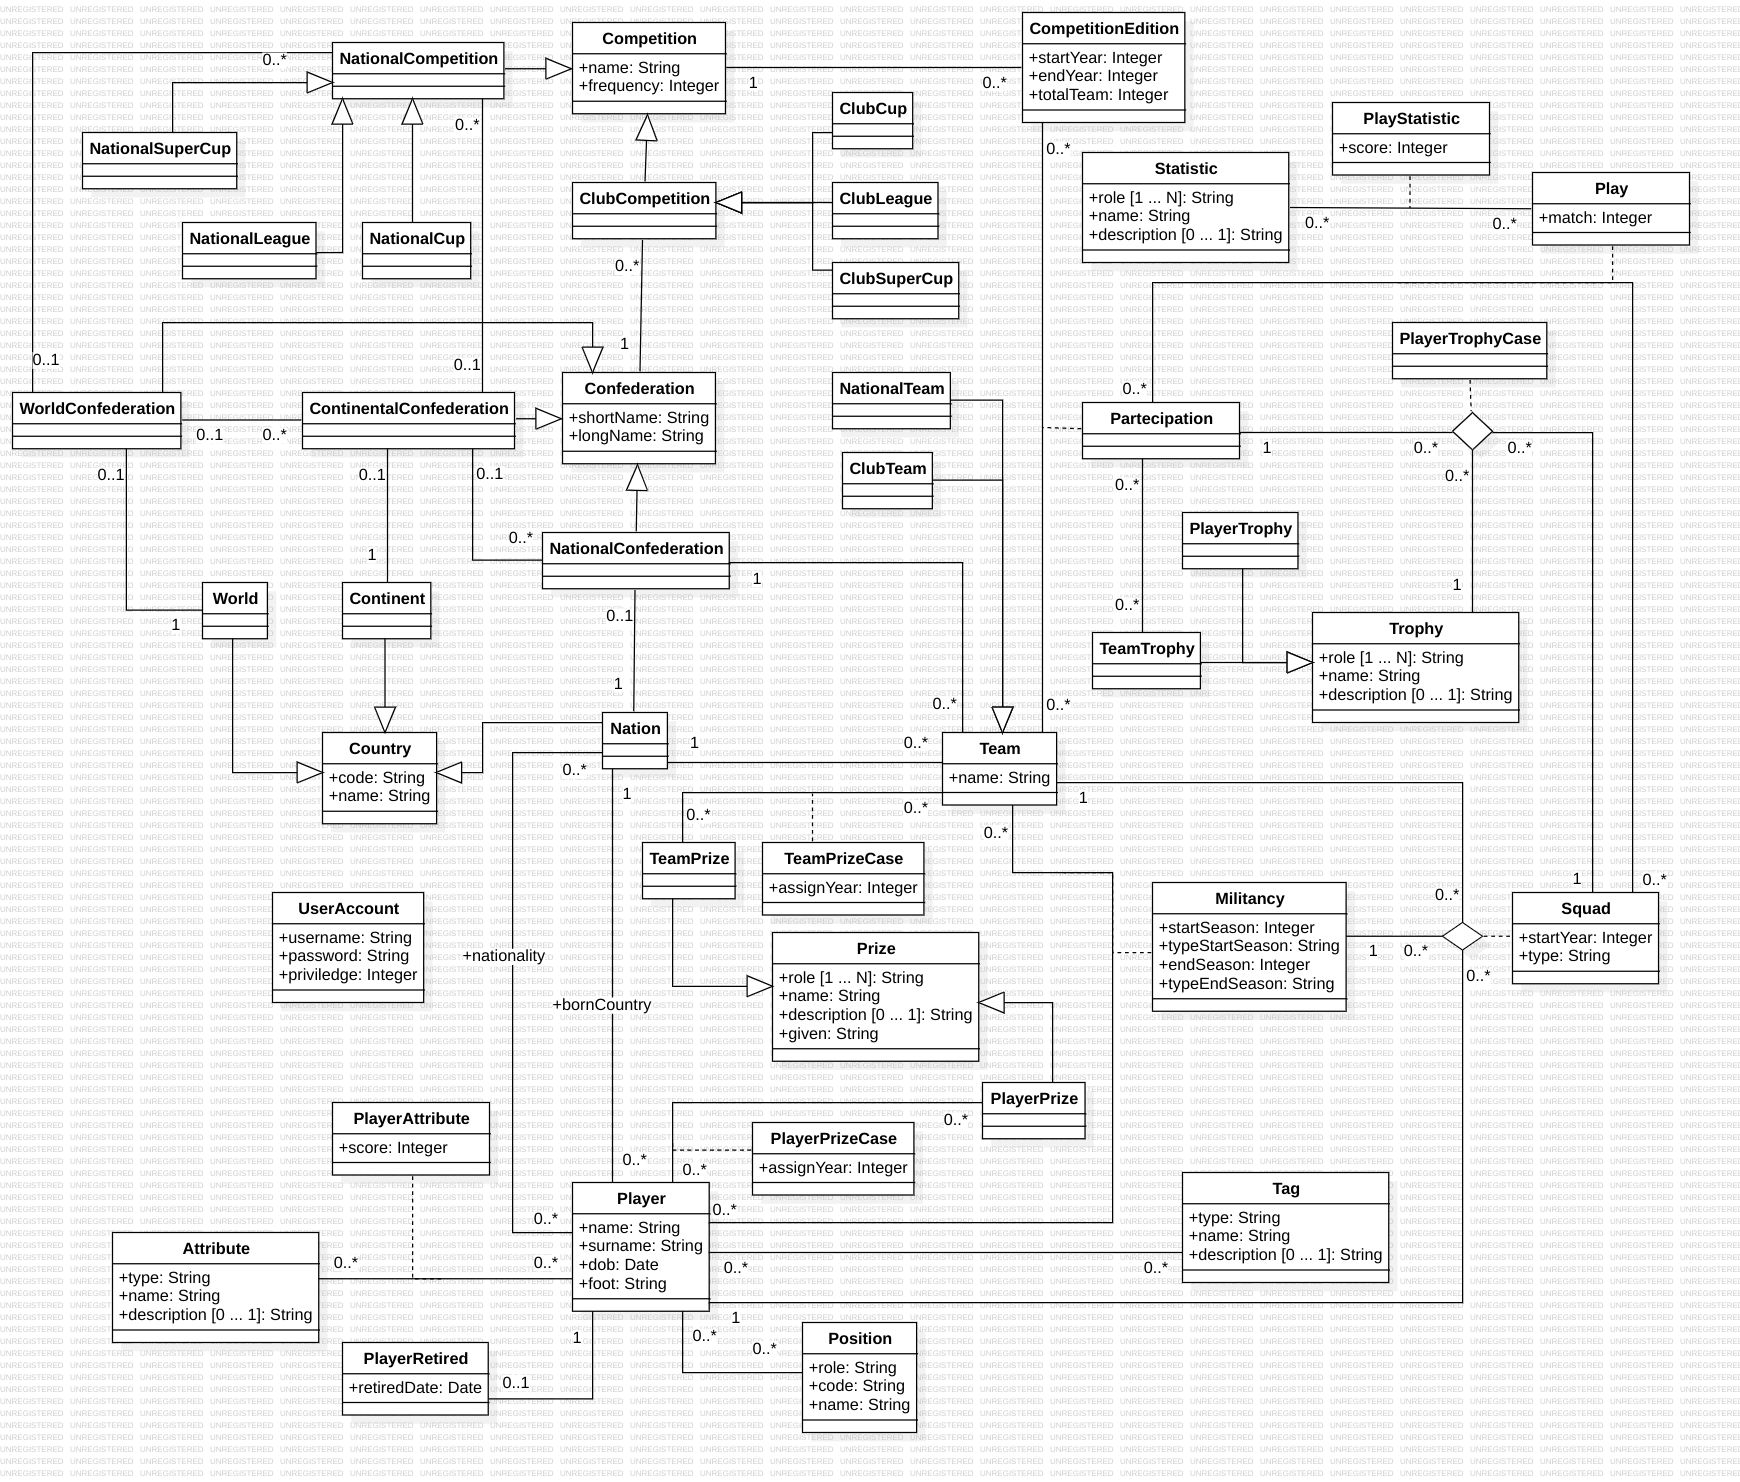
\includegraphics[width=\textwidth]{res/class_diagram_not_restr}
\newpage

\subsubsection{\Large Ristrutturazione del Class Diagram}

\textbf{\large Analisi delle Ridondanze}

Possiamo constatare che non ci sono attributi ridondanti.

Notiamo però che vista l'alta frequenza di certe operazioni, 
che dovranno essere compiute sul database, vi è
un impellente necessità di introdurre delle ridondanze.


Prima operazione su tutte, è la visualizzazione di un 
resoconto delle statistiche di un calciatore rispetto alla 
sua militanza
(operazione richiesta anche dalla traccia).
Quest'ultimo infatti si potrebbe ottenere facendo una somma 
delle  statistiche riferite ai Play che sono associati allo 
specifico calciatore, alla squadra della militanza che si sta 
tenendo in considerazione e che siano avvenuti nell'arco di 
tempo in cui il calciatore in questione militava per quella 
certa squadra.


Per evitare che ad ogni richiesta di questa operazione si 
debba rifare il calcolo, soffermandoci nuovamente sul fatto 
che si suppone che questa operazione venga effettuata un 
numero molto elevato di volte, si vede la necessità di 
aggiungere in \textbf{Militanza} un attributo \textbf{match} 
che conservi il numero di presenze in campo di un calciatore 
durante quella specifica militanza.

Inoltre, vi è necessario aggiungere una classe 
\textbf{MilitancyStatistic} che sarà associata a 
\textbf{Statistic} e a \textbf{Militancy}, e che conterrà 
come attributo, \textbf{score} che ha lo scopo di conservare 
il valore di una certa statistica di un calciatore durante 
una specifica militanza.


Un'altra operazione che si suppone sia ricorrente, è il 
resoconto
del numero di presenze in campo di un calciatore in una 
determinata posizione.
Questo calcolo si potrebbe ottere dalla somma dell'attributo 
\textbf{match} delle tuple in Play associate al calciatore in 
quella determinata posizione.

Per velocizzare l'operzione si vede necessario, dunque, 
introdurre nella classe \textbf{PlayPosition} un attributo 
\textbf{match} che conservi il numero di presenze in campo di 
un calciatore in una specifica posizione.


L'ultima operazione, ovvero la visualizzazione delle 
nazionalità di un giocatore, si potrebbe ottenere navigando 
entrambe le associazioni che \textbf{Player} ha con 
\textbf{Country}: bornCountry e Nationality.

Visto che il nostro database ha come scopo primario l'essere 
un sistema informativo per i calciatori, si vede necessario 
aggiungere alla relazione Nationality anche la nazione di 
nascita del calciatore così da velocizzare l'operazione, in 
quanto così facendo basta navigare soltanto l'associazione 
Nationality.

\newpage
\textbf{\large Eliminazione delle Generalizzazioni}

Nonostante le numerose generalizzazioni presenti nel Class 
Diagram, tutte hanno un qualcosa in comune, ovvero sono 
generalizzazioni disgiunte totali, e in particolare le classi 
figlie non hanno attributi propri, ma al massimo associazioni 
con altre classi.

A seguito di ciò dunque, come metodo per eliminarle, si 
deciso di adottare l'accorpamento delle figlie della 
generalizzazione nel padre, aggiungendo dove necessario un 
attributo \textbf{type} che distinguesse le varie istanze 
della classe padre, e facendo le dovute correzioni ad 
eventuali associazioni delle classi figlie con le altre 
classi.

Di seguito viene mostrato un elenco delle generalizzazioni e 
di come sono state ristrutturate:

\bigskip
\textbf{Country}
\bigskip

Alla classe \textbf{Country} è stato aggiunto un attributo 
\textbf{type} di tipo enum chiamato \textbf{enCountry}.
Il tipo \textbf{enCountry} può assumere tre valori:
\begin{itemize}
	\item Nation;
	\item Continental;
	\item World.
\end{itemize}

Per quanto riguarda le associazioni:

Le associazioni delle classi figlie di \textbf{Country} con 
le classi figlie di \textbf{Confederation} sono state 
accorpate, risultandone in un unica associazione tra 
\textbf{Country} e \textbf{Confederation} con molteplicità 
invariata.

Per quanto riguarda le associazioni della classe figlia 
\textbf{Nation} con \textbf{Player} e \textbf{Team}, esse 
sono state ricollegate alla classe padre \textbf{Country} 
mantenendo la molteplicità invariata.

\bigskip
\textbf{Confederation}
\bigskip

Alla classe \textbf{Confederation}  non è stato aggiunto un 
attributo \textbf{type} poiché si è sfruttato l'associazione 
1 a 1 che le classi figlie di \textbf{Confederation} avevano 
con le classi figlie di \textbf{Country}.
Dunque per comprendere a quale classe figlia una tupla di 
\textbf{Confederation} corrisponde, bisogna basarsi 
sull'attributo \textbf{type} della classe \textbf{Country}.

Per quanto riguarda le associazioni:

Le due associazioni che intercorrono tra le classi figlie di 
\textbf{Confederation}, ovvero l'associazione tra 
\textbf{NationalConfederation} e 
\textbf{ContinentalConfederation}, e tra 
\textbf{ContinentalConfederation} e 
\textbf{WorldConfederation}, sono state accorpate, 
risultandone in un'unica associazione tra la classe 
\textbf{Confederation} e sé stessa.

Le due associazioni delle classi figlie 
\textbf{ContinentalConfederation} e 
\textbf{WorldConfederation} con \textbf{NationalCompetition}, 
sono state accorpate, risultandone in un'unica associazione 
tra la classe \textbf{Confederation} e la classe 
\textbf{Competition}, classe padre di 
\textbf{NationalCompetition}.

\newpage
\textbf{Competition}
\bigskip

Alla classe \textbf{Competition} sono stati aggiunti due 
attributi: \textbf{type} di tipo enum chiamato 
\textbf{enCompetition} e \textbf{teamType} di tipo enum 
chiamato \textbf{enTeam}. Questo perché anche le classi 
figlie di \textbf{Competition} erano una generalizzazione a 
loro volta.

Nota che ci si è ridotti a solo due tipi aggiunti, perché le 
classi \textbf{NationalCompetition} e {ClubCompetition} hanno 
le stesse classi figlie.

Il tipo enum \textbf{enTeam} può assumere i seguenti valori:
\begin{itemize}
	\item National;
	\item Club.
\end{itemize}

Il tipo enum \textbf{enCompetition} può assumere i seguenti 
valori:
\begin{itemize}
	\item Cup;
	\item League;
	\item Super Cup.
\end{itemize}

Per quanto riguarda le associazioni:

L'associazione tra \textbf{ClubCompetition} e 
\textbf{Confederation}, è stata ricollegata alla classe padre 
\textbf{Competition} mantenendone però la molteplicità 
invariata.


Le associazioni tra \textbf{NationalCompetition} e  
\textbf{NationalCompetitionEdition} e tra 
\textbf{ClubCompetition} e \textbf{ClubCompetitionEdition} 
sono state accorpate, risultandone in un'unica associazione 
(con molteplicità invariata) tra \textbf{Competition} e 
\textbf{CompetitionEdition}, la classe padre di 
\textbf{NationalCompetitionEdition} e 
\textbf{ClubCompetitionEdition}.

\bigskip
\textbf{CompetitionEdition}
\bigskip

Alla classe \textbf{CompetitionEdition} non è stato aggiunto 
un attributo \textbf{type} poiché si è sfruttata 
l'associazione che vi era tra le sue classi figlie e le 
classi figlie di \textbf{Competition}. Dunque per comprendere 
a quale classe figlia una tupla di 
\textbf{CompetitionEdition} corrisponde, bisogna basarsi 
sull'attributo \textbf{teamType} della classe 
\textbf{Competition}.

Per quando riguarda le associazioni:

Le associazioni tra \textbf{NationalCompetitionEdition} e 
\textbf{NationalPartecipation} e tra 
\textbf{ClubCompetitionEditon} e \textbf{ClubPartecipation}, 
sono state accorpate, risultandone in un'unica associazione 
(con molteplicità invariata) tra la classe 
\textbf{CompetitionEdition} e \textbf{Partecipation}, la 
classe padre di \textbf{NationalPartecipation} e 
\textbf{ClubPartecipation}.


\bigskip
\textbf{Team}
\bigskip

Alla classe \textbf{Team} è stato aggiunto un attributo 
\textbf{type} di tipo enum chiamato \textbf{enTeam} (lo 
stesso di Competition).

Per quanto riguarda le associazioni:

Le associazioni tra \textbf{National} e 
\textbf{NationalPartecipation} e tra \textbf{Club} e 
\textbf{ClubPartecipation}, sono state accorpate, 
risultandone in un'unica associazione tra la classe 
\textbf{Team} e \textbf{Partecipation} la classe padre di
\textbf{NationalPartecipation} e \textbf{ClubPartecipation}


\newpage

\textbf{Partecipation}
\bigskip

Alla classe \textbf{Partecipation} non è stato aggiunto un 
attributo \textbf{type} poiché si è sfruttata l'associazione 
che vi era tra le sue classi figlie e le classi figlie di 
\textbf{Team}. Dunque per comprendere a quale classe figlia 
una tupla di \textbf{Partecipation} corrisponde, bisogna 
basarsi sull'attributo \textbf{type} della classe 
\textbf{Team}.

Per quanto riguarda le associazioni:
Sono già state gestite precedentemente.

\bigskip
\textbf{Trophy}
\bigskip

Alla classe \textbf{Trophy} è stato aggiunto un attributo 
\textbf{type} di tipo enum chiamato \textbf{enAward}.

Il tipo \textbf{enAward} assume i seguenti valori:
\begin{itemize}
	\item Player
	\item Team
\end{itemize}


Per quanto riguarda le associazioni:

L'associazione tra \textbf{TeamTrophy} e 
\textbf{Partecipation} è stata ricollegata alla classe padre 
\textbf{Trophy} mantenendo la molteplicità invariata.


\bigskip
\textbf{Prize}
\bigskip

Alla classe \textbf{Prize} è stato aggiunto un attributo 
\textbf{type} di tipo enum chiamato \textbf{enAward} (lo 
stesso tipo di Trophy).

Per quanto riguarda le associazioni:

L'associazione tra \textbf{TeamPrize} e 
\textbf{TeamPrizeCase} è stata ricollegata alla classe padre 
\textbf{Prize} mantenendo la molteplicità invariata.


L'associazione tra \textbf{PlayerPrize} e 
\textbf{PlayerPrizeCase} è stata ricollegata alla classe 
padre \textbf{Prize} mantenendo la molteplicità invariata.

\bigskip
\textbf{\large Eliminazioni Attributi Multivalore}
\bigskip

Vi sono tre attributi multivalore presenti nel Class Diagram:
\begin{itemize}
	\item L'attributo \textbf{role}
		della classe \textbf{Prize};
	\item L'attributo \textbf{role}
		della classe \textbf{Trophy};
	\item L'attributo \textbf{role}
		della classe \textbf{Statistic}.
\end{itemize}

Questo attributo assume la stessa funzione in tutte e tre le 
Classi, ovvero quello di descrivere quella determinata classe 
a quali ruoli può essere associata.


Data l'importanza assunta da quest'attributo, si è deciso di 
creare un tipo enum che contiene tutte le combinazioni di 
ruoli possibili (ci possono essere massimo 4 ruoli).

\newpage
\textbf{\large Eliminazione Attributi Strutturati}
\bigskip

Nel Class Diagram non sono presenti Attributi Strutturati.

\bigskip
\textbf{\large Partizionamento/Accorpamento di Entità
		e Associazioni}
\bigskip

L'unica accorpamento che potrebbe essere effettuato nel Class 
Diagram è quello tra \textbf{Country} e 
\textbf{Confederation}, poiché tra esse vi è un'associazione 
1 a 1.

Si è arrivati però alla conclusione che c'è bisogno che le 
due classi siano separate, perché nelle altre associazioni 
che esse hanno con le altre classi, svolgono un ruolo 
centrale.

\bigskip
\textbf{\large Scelta degli Identificatori Primari}
\bigskip

\newpage
\subsubsection{\Large Class Diagram ristrutturato}
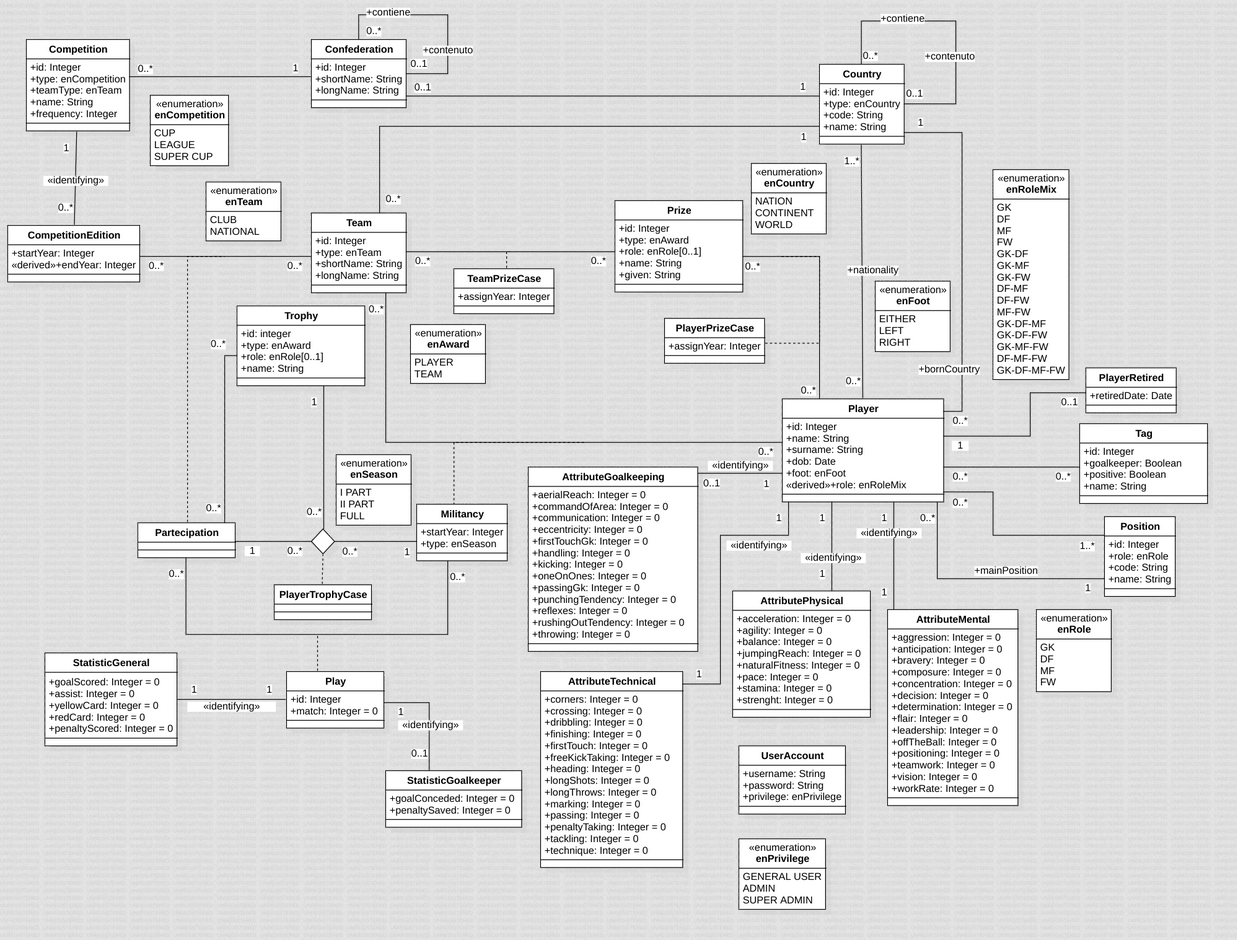
\includegraphics[scale= 0.242]{res/class_diagram_ristr}
\newpage

\subsubsection{\Large Dizionario}

\begin{center}
	\textbf{Dizionario delle Classi}
\end{center}


\begin{tblr}{
    hlines = {0.9pt}, vlines = {0.9pt}, colspec = {X[l]X[l]X[l]}, column{1}= {100pt},
    width = \textwidth, cell{1}{1-3} = {blue!10!white}
}
	{
		Classe
	}
	&
	{
		Descrizione
	}
	&
	{
		Attributo
	}
	\\
	{
		Attribute
	}
	&
	{
		Rappresenta gli attributi di un calciatore.
	}
	&
	{
		\textbf{id}(Integer)[chiave surrogata]:\\Rappresenta
			l'identificativo di un Attributo.\\
		\medskip\textbf{type}(enFeature):\\Rappresenta
			il tipo di un Attributo.\\
		\medskip\textbf{name}(String)[chiave naturale]:
			\\Rappresenta il nome di un Attributo.\\
		\medskip\textbf{description}(String)[parziale]:
			\\Rappresenta la descrizione di un Attributo.
	}
	\\
	{
		Competition
	}
	&
	{
		Rappresenta le competizioni calcistiche.
	}
	&
	{
		\textbf{id}(Integer)[chiave surrogata]:\\Rappresenta
			l'identificativo di una Competizione.\\
		\medskip\textbf{type}(enCompetition):\\Rappresenta
			il tipo di una Competizione.\\
		\medskip\textbf{teamType}(enTeam):\\Rappresenta
			il tipo di squadra che può
			partecipare alla Competizione.\\
		\medskip\textbf{name}(String)[chiave naturale]:
			\\Rappresenta il nome di una Competizione.\\
		\medskip\textbf{frequency}(Integer):\\Rappresenta
			la frequenza di una Competizione.
	}
	\\
	{
		CompetitionEdition
	}
	&
	{
		Rappresenta le edizioni delle competizioni calcistiche.
	}
	&
	{
		\textbf{id}(Integer)[chiave surrogata]:\\Rappresenta
			l'identificativo di un'Edizione.\\
		\medskip\textbf{startYear}(Integer)[chiave parziale]:
			\\Rappresenta l'anno di inizio di un'Edizione.\\
		\medskip\textbf{endYear}(Integer)[chiave parziale]:
			\\Rappresenta l'anno di fine di un'Edizione.\\
		\medskip\textbf{totalTeam}(Integer):\\Rappresenta
			il numero di team che partecipano in un'Edizione.
	}
	\\
	{
		Confederation
	}
	&
	{
	Rappresenta le confederazioni calcistiche.
	}
	& 
	{
		\textbf{id}(Integer)[chiave surrogata]:\\Rappresenta
			l'identificativo di una Confederazione.\\
		\medskip\textbf{shortName}(String):\\Rappresenta
			il nome abbreviato di una Confederazione.\\
		\medskip\textbf{longName}(String)[chiave naturale]:
			\\Rappresenta il nome esteso di una Confederazione.
	}
	\\
\end{tblr}

\newpage

\begin{tblr}{
    hlines = {0.9pt}, vlines = {0.9pt}, colspec = {X[l]X[l]X[l]}, column{1}= {100pt},
    width = \textwidth
}
	{
		Country
	}
	&
	{
		Rappresenta i paesi in cui si gioca
		ufficialmente a calcio.
	}
	&
	{
		\textbf{id}(Integer)[chiave surrogata]:\\Rappresenta
			l'identificativo di un Paese.\\
		\medskip\textbf{type}(enCountry):\\Rappresenta
			il tipo di un Paese.\\
		\medskip\textbf{code}(String)[chiave naturale]:
			\\Rappresenta il codice ISO 3166-1 alpha-3
			di un Paese.\\
		\medskip\textbf{name}(String)[chiave naturale]:
			\\Rappresenta il nome di un Paese.
	}
	\\
	{
		Militancy
	}
	&
	{
		Rappresenta le militanze di un
		calciatore in una squadra.
	}
	&
	{
		\textbf{id}(Integer)[chiave surrogata]:\\Rappresenta
			l'identificativo di una Militanza.\\
		\medskip\textbf{dateRange}(daterange):\\Rappresenta
			il periodo di tempo in cui
			un calciatore era nella squadra.\\
		\medskip\textbf{match}(Integer)[derivato]:\\Rappresenta
			il numero di presenze di un Calciatore.
	}
	\\
	{
		MilitancyStatistic
	}
	&
	{
		Rappresenta l'associazione tra
		Militancy e Statistic.\\È una classe associativa.
	}
	& 
	{
		\textbf{score}(Integer)[derivato]:\\Rappresenta
			il valore di una Statistica per
			la Militanza associata.
	}
	\\
	{
		Partecipation
	}
	&
	{
		Rappresenta la partecipazione
		di un Team ad una CompetitionEdition.\\
		È una classe associativa.
	}
	&
	{
	
	}
	\\
	{
		Play
	}
	&
	{
		Rappresenta l'associazione tra
		Partecipation e PlayerPosition.\\
		È una classe associativa.
	}
	&
	{
		\textbf{id}(Integer)[chiave surrogata]:\\Rappresenta
			l'identificativo di un Gioco.\\
		\medskip\textbf{match}(Integer):\\Rappresenta
			il numero di presenze del Calciatore
			in quella Posizione, in una Squadra, per quella
			Edizione della competizione.
	}
	\\
	{
		PlayStatistic
	}
	&
	{	
		Rappresenta l'associazione tra Play e Statistic.\\
		È una classe associativa.
	}
	&
	{
		\textbf{score}(Integer):\\Rappresenta
			il valore di una Statistica per il Play associato.
	}
	\\
	{
		Player
	}
	&
	{
		Rappresenta i calciatori.
	}
	&
	{
		\textbf{id}(Integer)[chiave surrogata]:\\Rappresenta
			l'identificativo di un Calciatore.\\
		\medskip\textbf{name}(String):\\Rappresenta
			il nome di un Calciatore.\\
		\medskip\textbf{surname}(String):\\Rappresenta
			il cognome di un Calciatore.\\
		\medskip\textbf{dob}(Date):\\Rappresenta
			la data di nascita.\\
		\medskip\textbf{foot}(enFoot):\\Rappresenta
			il piede preferito di un Calciatore.\\
		\medskip\textbf{careerTime}(daterange):\\Rappresenta
			l'intervallo di tempo tra la data di debutto
			e la data di ritiro di un Calciatore.
	}
	\\
\end{tblr}

\newpage

\begin{tblr}{
    hlines = {0.9pt}, vlines = {0.9pt}, colspec = {X[l]X[l]X[l]}, column{1}= {100pt},
    width = \textwidth
}

	{
		PlayerAttribute
	}
	&
	{
		Rappresenta l'associazione tra Player e Attribute.\\
		È una classe associativa.
	}
	&
	{
		\textbf{score}(Integer):\\Rappresenta
			il valore di un Attributo associato al Calciatore.
	}
	\\
	{
		PlayerPosition
	}
	&
	{
		Rappresenta l'associazione tra Player e Position.\\
		È una classe associativa.
	}
	&
	{
		\textbf{match}(Integer)[derivato]:\\Rappresenta
			il numero di partite che un Calciatore gioca
			in una determinata Posizione.
	}
	\\
	{
		PlayerPrizeCase
	}
	&
	{
		Rappresenta la bacheca dei premi del calciatore.
	}
	&
	{
		\textbf{assignYear}(Integer):\\Rappresenta
			l'anno di assegnazione di un Premio.
	}
	\\
	{
		PlayerTrophyCase
	}
	&
	{
		Rappresenta la bacheca dei trofei di un calciatore.
	}
	&
	{
	
	}
	\\
	{
		Position
	}
	&
	{
		Rappresenta le posizioni di gioco di un Calciatore.
	}
	&
	{
		\textbf{id}(Integer)[chiave surrogata]:\\Rappresenta
			l'identificativo di una Posizione.\\
		\medskip\textbf{role}(enRole):\\Rappresenta
			il ruolo associato ad una Posizione.\\
		\medskip\textbf{code}(String)[chiave naturale]:
			\\Rappresenta il nome abbreviato di una Posizione.\\
		\medskip\textbf{name}(String)[chiave naturale]:
			\\Rappresenta il nome di una Posizione.
	}
	\\
	{
		Prize
	}
	&
	{
		Rappresenta i premi calcistici.
	}
	&
	{
		\textbf{id}(Integer)[chiave surrogata]:\\Rappresenta
			l'identificativo del Premio.\\
		\medskip\textbf{type}(enAward):\\Rappresenta
			il tipo del Premio.\\
		\medskip\textbf{role}(enRoleMix):\\Rappresenta
			i possibili ruoli che sono associati ad un Premio.\\
		\medskip\textbf{name}(String)[chiave naturale]:
			\\Rappresenta il nome del Premio.\\
		\medskip\textbf{description}(String)[parziale]:
			\\Rappresenta la descrizione del Premio.\\
		\medskip\textbf{given}(String):\\Rappresenta
			il nome della società calcistica
			che conferisce il Premio.
	}
	\\
	{
		Statistic
	}
	&
	{
		Rappresenta le statistiche di un calciatore.
	}
	&
	{
		\textbf{id}(Integer)[chiave surrogata]:\\Rappresenta
			l'identificativo della Statistica.\\
		\medskip\textbf{role}(enRoleMix):\\Rappresenta
			i ruoli associati alla Statistica.\\
		\medskip\textbf{name}(String):\\Rappresenta
			il nome della Statistica.\\
		\medskip\textbf{description}(String)[parziale]:
			\\Rappresenta la descrizione della Statistica.
	}
	\\
\end{tblr}

\newpage

\begin{tblr}{
    hlines = {0.9pt}, vlines = {0.9pt}, colspec = {X[l]X[l]X[l]}, column{1}= {100pt},
    width = \textwidth
}
	{
		Tag
	}
	&
	{
		Rappresenta i tag di un calciatore.
	}
	&
	{
		\textbf{id}(Integer)[chiave surrogata]:\\Rappresenta
			l'identificativo del Tag.\\
		\medskip\textbf{type}(enFeature):\\Rappresenta
			il tipo del Tag.\\
		\medskip\textbf{name}(String)[chiave naturale]:
			\\Rappresenta il nome del Tag.\\
		\medskip\textbf{description}(String)[parziale]:
			\\Rappresenta la descrizione del Tag.
	}
	\\
	{
		Team
	}
	&
	{
		Rappresenta le squadre di calcio.
	}
	&
	{
		\textbf{id}(Integer)[chiave surrogata]:\\Rappresenta
			l'identificativo della Squadra.\\
		\medskip\textbf{type}(enTeam):\\Rappresenta
			il tipo della Squadra.\\
		\medskip\textbf{name}(String)[chiave naturale]:
			\\Rappresenta il nome della Squadra.
	}
	\\
	{
		TeamPrizeCase
	}
	&
	{
		Rappresenta la bacheca dei premi della squadra.
	}
	&
	{
		\textbf{assignYear}(Integer):\\Rappresenta
			l'anno di assegnazione di un Premio.
	}
	\\
	{
		Trophy
	}
	&
	{
		Rappresenta i trofei calcistici.
	}
	&
	{
		\textbf{id}(Integer)[chiave surrogata]:\\Rappresenta
			l'identificativo del Trofeo.\\
		\medskip\textbf{type}(enAward):\\Rappresenta
			il tipo del Trofeo.\\
		\medskip\textbf{role}(enRoleMix):\\Rappresenta
			i possibili ruoli a cui è associato un Trofeo.\\
		\medskip\textbf{name}(String)[chiave naturale]:
			\\Rappresenta il nome del Trofeo.\\
		\medskip\textbf{description}(String)[parziale]:
			\\Rappresenta la descrizione del Trofeo.\\
	}
	\\
	{
		UserAccount
	}
	&
	{
		Rappresenta gli utenti dell'applicativo.
	}
	&
	{
		\textbf{username}(String)[chiave naturale]:\\Rappresenta
			l'username dell'Account dell'Utente.\\
		\medskip\textbf{password}(String):\\Rappresenta
			la password dell'Account dell'Utente.\\
		\medskip\textbf{priviledge}(Integer):\\Rappresenta
			i privilegi dell'Account dell'Utente.
	}
	\\
\end{tblr}

\newpage

\begin{center}
	\textbf{Dizionario delle Associazioni}
\end{center}


\begin{tblr}{
    hlines = {0.9pt}, vlines = {0.9pt}, colspec = {X[l]X[l]X[l]}, column{1}= {100pt},
    width = \textwidth, cell{1}{1-3} = {blue!10!white}
}

	{
		Nome
	}
	&
	{
		Descrizione
	}
	&
	{
		Classi in Relazione
	}
	\\
	{
		Nationality
	}
	&
	{
		Esprime le nazionalità di un calciatore.
	}
	&
	{
		\textbf{Country [0 ... *]}:\\Indica che
			uno stesso paese può essere associato a più
			calciatore.\\
		\medskip\textbf{Player [0 ... *]}:\\Indica che
			un calciatore può avere più nazionalità.
	}
	\\
	{
		bornCountry	
	}
	&
	{
		Esprime il paese di nascita di un calciatore.
	}
	&
	{
		\textbf{Country [0 ... *]}:\\Indica che
			un paese può essere il paese di nascita
			di più calciatori.\\
		\medskip\textbf{Player [1]}:\\Indica che
			un calciatore ha uno e un solo paese di nascita.
	}
	\\
	{
		\textbf{Player-PlayerAttribute}
	}
	&
	{
		Esprime il valore degli attributi di un calciatore.
	}
	&
	{
		\textbf{Player [0 ... *]}:\\Indica che un Calciatore
			può aver zero o più valori di Attributi associati.\\
		\medskip\textbf{PlayerAttribute [1]}:\\Indica che 
			un valore di un Attributo deve essere associato
			ad uno e un solo Calciatore.
	}
	\\
	{
		\textbf{PlayerAttribute-Attribute}
	}
	&
	{
		Esprime a quale attributo si riferisce
		PlayerAttribute.
	}
	&
	{
		\textbf{PlayerAttribute [1]}:\\Indica che un valore
			di PlayerAttribute è associato ad uno e un solo
			Attributo.\\
		\medskip\textbf{Attribute [0 ... *]}:\\Indica che un
			Attributo può avere più valori associati.
	}
	\\
	{
		\textbf{Player-Tag}
	}
	&
	{
		Esprime i Tag associati ad un Calciatore.
	}
	&
	{
		\textbf{Player [0 ... *]}:\\Indica che un Calciatore
			può avere più Tag associati.\\
		\medskip\textbf{Tag [0 ... *]}:\\Indica che
			uno stesso Tag può essere associato a
			più Calciatori.
	}
	\\
	{
		\textbf{Player-PlayerTrophyCase}
	}
	&
	{
		Esprime i trofei associati ad un calciatore.
	}	
	&
	{
		\textbf{Player [0 ... *]}:\\Indica che un Calciatore
			può avere più Trofei associati.\\
		\medskip\textbf{PlayerTrophyCase [1]}:\\Indica che una
			bacheca si può riferire ad uno e un solo Calciatore.
	}
	\\
	{
		\textbf{PlayerTrophyCase-Trophy}
	}
	&
	{
		Esprime i trofei associati ad una bacheca.
	}
	&
	{
		\textbf{PlayerTrophyCase [1]}:\\Indica che una bacheca
			si può riferire ad uno e un solo Trofeo.\\
		\medskip\textbf{Trophy [0 ... *]}:\\Indica che
			un Trofeo può avere più bacheche associate.
	}
	\\
\end{tblr}

\newpage

\begin{tblr}{
    hlines = {0.9pt}, vlines = {0.9pt}, colspec = {X[l]X[l]X[l]}, column{1}= {100pt},
    width = \textwidth
}

	{
		\textbf{PlayerTrophyCase-Partecipation}
	}
	&
	{
		Esprime le partecipazioni di una squadra
		ad una competizione edizione associate
		ad una bacheca.
	}
	&
	{
		\textbf{PlayerTrophyCase [1]}:\\Indica che una bacheca
			si può riferire ad uno e un sola Partecipazione.\\
		\medskip\textbf{Partecipation [0 ... *]}:\\Indica che
			una Partecipazione può avere più bacheche associate.
	}
	\\
	{
		\textbf{Player-PlayerPosition}
	}
	&
	{
		Esprime il numero di partite che un Calciatore
		ha fatto in una certa posizione.
		
	}
	&
	{
		\textbf{Player [0 ... *]}:\\Indica che un Calciatore
			può avere più posizioni di gioco associate.\\
		\medskip\textbf{PlayerPosition [1]}:\\Indica che
			il numero di partite di una posizione di gioco si
			può riferire ad uno e un solo Calciatore.
	}
	\\
	{
		\textbf{PlayerPosition-Position}
	}
	&
	{
		Esprime a quale posizione è associato
		il numero di partite di un Calciatore.
	}
	&
	{
		\textbf{PlayerPosition [1]}:\\Indica che il numero
			di partite di una posizione di gioco si può riferire
			ad una e una sola posizione.\\
		\medskip\textbf{Position [0 ... *]}:\\Indica che
			una Posizione può avere più calciatori associati.
	}
	\\
	{
		\textbf{Player-Militancy}
	}
	&
	{
		Esprime le Militanze associate ad un Calciatore.
	}
	&
	{
		\textbf{Player [0 ... *]}:\\Indica che il Calciatore
			può avere più Militanze associate.\\
		\medskip\textbf{Militancy [1]}:\\Indica che
			una Militanza si può riferire ad uno
			e un solo Calciatore.
	}
	\\
	{
		\textbf{Militancy-Team}
	}
	&
	{
		Esprime a quale Squadra una Militanza è associata.
	}
	&
	{
		\textbf{Militancy [1]}:\\Indica che una Militanza
			si può riferire ad una e una sola Squadra.\\
		\medskip\textbf{Team [0 ... *]}:\\Indica che una Squadra
			può avere più Militanze associate.
	}
	\\
	{
		\textbf{Player-PlayerPrizeCase}
	}
	&
	{
		Esprime i premi associati ad un Calciatore
		nella Bacheca.
	}
	&
	{
		\textbf{Player [0 ... *]}:\\Indica che un Calciatore
			può avere più premi associati in una Bacheca.\\
		\medskip\textbf{PlayerPrizeCase [1]}:\\Indica che una
			Bacheca si può riferire ad un e un solo Calciatore.
	}
	\\
	{
		\textbf{PlayerPrizeCase-Prize}
	}
	&
	{
		Esprime i Premi ai quali è associata una Bacheca.
	}
	&
	{
		\textbf{PlayerPrizeCase [1]}:\\Indica che una Bacheca
			si può riferire ad un e un solo Premio.\\
		\medskip\textbf{Prize [0 ... *]}:\\Indica che un Premio
			può avere più Bacheche associate.
	}
	\\
	{
		\textbf{Team-Country}
	}
	&
	{
		Esprime la nazionalità di una Squadra.
	}
	&
	{
		\textbf{Team [1]}:\\Indica che una Squadra si riferisce
			ad un e un solo paese.\\
		\medskip\textbf{Country [0 ... *]}:\\Indica che un Paese
			può avere più Squadre associate.
	}
	\\
\end{tblr}

\newpage

\begin{tblr}{
    hlines = {0.9pt}, vlines = {0.9pt}, colspec = {X[l]X[l]X[l]}, column{1}= {100pt},
    width = \textwidth
}

	{
		\textbf{Team-Confederation}
	}
	&
	{
		Esprime la Confederazione di cui una Squadra è membra.
	}
	&
	{
		\textbf{Team [1]}:\\Indica che una Squadra si riferisce
			ad una e una sola Confederazione.\\
		\medskip\textbf{Confederation [0 ... *]}:\\Indica che
			una Confederazione può avere più Squadre associate.
	}
	\\
	{
		\textbf{Team-Partecipation}
	}
	&
	{
		Esprime le edizioni delle Competizioni a cui una Squadra
		Partecipa.
	}
	&
	{
		\textbf{Team [0 ... *]}:\\Indica che una Squadra può
			partecipare a più Competizioni Edizioni.\\
		\medskip\textbf{Partecipation [1]}:\\Indica che una
			Partecipazione può riferirsi ad una e una sola
			Squadra.
	}
	\\
	{
		\textbf{Partecipation-CompetitionEdition}
	}
	&
	{
		Esprime a quali Edizioni di una Competizione una
		Partecipazione di una Squadra si riferisce.
	}
	&
	{
		\textbf{Partecipation [1]}:\\Indica che
			una Partecipazione può riferirsi ad una e una sola
			Edizione di una Competizione.\\
		\medskip\textbf{CompetitionEdition [0 ... *]}:\\Indica
			che una Edizione di una Competizione può avere più
			Partecipazioni associate.
	}
	\\
	{
		\textbf{Team-TeamPrizeCase}
	}
	&
	{
		Esprime i premi associati ad una Squadra
		in una Bacheca.
	}
	&
	{
		\textbf{Team [0 ... *]}:\\Indica che una Squadra
			può avere più premi associati in una Bacheca.\\
		\medskip\textbf{TeamPrizeCase [1]}:\\Indica che una
			Bacheca si può riferire ad una e una sola Squadra.
	}
	\\
	{
		\textbf{TeamPrizeCase-Prize}
	}
	&
	{
		Esprime i Premi ai quali è associata una Bacheca.
	}
	&
	{
		\textbf{TeamPrizeCase [1]}:\\Indica che una Bacheca
			si può riferire ad un e un solo Premio.\\
		\medskip\textbf{Prize [0 ... *]}:\\Indica che un Premio
			può avere più Bacheche associate.
	}
	\\
	{
		\textbf{Confederation-Country}
	}
	&
	{
		Esprime l'appartenza di una Confederazione
		ad un unico Paese.
	}
	&
	{
		\textbf{Confederation [1]}:\\Indica che
			una Confederazione si può riferire
			ad un e un solo Paese.\\
		\medskip\textbf{Country [0 ... 1]}:\\Indica che
			un Paese si può riferire a nessuna o ad una
			Confederazione.
	}
	\\
	{
		Membro
	}
	&
	{
		Esprime la possibilità di una confederazione di
		avere come membri altre confederazioni, o essere
		membro a sua volta.
	}
	&
	{
		\textbf{Confederation [0 ... 1]} ruolo (contenuto):\\
			Indica che una Confederazione può o non può essere
			membra di un'altra Confederazione.\\
		\medskip\textbf{Confederation [0 ... *]}
			ruolo (contiene):\\
			Indica che una Confederazione può avere più
			Confederazioni come membri.
	}
	\\
	{
		\textbf{Confederation-Competition}
	}
	&
	{
		Esprime la capacità di una Confederazione di creare
		Competizioni.
	}
	&
	{
		\textbf{Confederation [0 ... *]}:\\Indica che una
			Confederazione può creare più Competizioni.\\
		\medskip\textbf{Competition [1]}:\\Indica che una
			Competizione si riferisce ad una e una sola
			Confederazione.
	}
	\\
\end{tblr}

\newpage

\begin{tblr}{
    hlines = {0.9pt}, vlines = {0.9pt}, colspec = {X[l]X[l]X[l]}, column{1}= {100pt},
    width = \textwidth
}
	{
		\textbf{Competition-CompetitionEdition}
	}
	&
	{
		Esprime la capacità di una Competizione di avere
		Edizioni.
		
	}
	&
	{
		\textbf{Competition [0 ... *]}:\\Indica che una
			Competizione può avere più Edizioni associate.\\
		\medskip\textbf{CompetitionEdition [1]}:\\Indica che
			una Edizione si riferisce ad una e una sola
			Competizione
	}
	\\
	{
		\textbf{Trophy-Partecipation}
	}
	&
	{
		Esprime la bacheca dei trofei di una Squadra.
	}
	&
	{
		\textbf{Trophy [0 ... *]}:\\Indica che un Trofeo
			può avere più Partecipazioni di una Squadra ad
			una Edizione associati.\\
		\medskip\textbf{Partecipation [0 ... *]}:\\Indica che
			una Partecipazione può avere più trofei associati.
	}
	\\
	{
		\textbf{Play-PlayerPosition}
	}
	&
	{
		Esprime un calciatore in che posizione ha giocato.
	}
	&
	{
		\textbf{Play [1]}:\\Indica che un Gioco si riferisce
			a una e una sola Posizione di gioco del Calciatore.\\
		\medskip\textbf{PlayerPosition [0 ... *]}:\\Indica che
			uno stesso Calciatore con la stessa
			Posizione di gioco può giocare più volte.
	}
	\\
	{
		\textbf{Play-Partecipation}
	}
	&
	{
		Esprime una squadra in che competizione ha giocato.
	}
	&
	{
		\textbf{Play [1]}:\\Indica che un Gioco si riferisce
			a una e una sola Partecipazione.\\
		\medskip\textbf{Partecipation [0 ... *]}:\\Indica che una
			Partecipazione può avere più Giochi associati.
	}
	\\
	{
		\textbf{Play-PlayStatistic}
	}
	&
	{
		Esprime la capacità di un Gioco di poter avere
		valori di Statistiche associati.
	}
	&
	{
		\textbf{Play [0 ... *]}:\\Indica che un Gioco può
			avere più valori di Statistiche associati.\\
		\medskip\textbf{PlayStatistic [1]}:\\Indica che
			il valore di una Statistica si riferisce ad
			uno e un solo Gioco.
	}
	\\
	{
		\textbf{PlayStatistic-Statistic}
	}
	&
	{
		Esprime la capacità delle Statistiche di poter avere
		più valori per il Gioco associati.
	}
	&
	{
		\textbf{PlayStatistic [1]}:\\Indica che un valore
			di una Statistica si riferisce ad una e una sola
			Statistica.\\
		\medskip\textbf{Statistic [0 ... *]}:\\Indica che
			una Statistica può avere più valori associati.
	}
	\\
	{
		\textbf{Statistic-MilitancyStatistic}
	}
	&
	{
		Esprime la capacità delle Statistiche di poter avere
		più valori per la Militanza associati.
	}
	&
	{
		\textbf{Statistic [0 ... *]}:\\Indica che una Statistica
			può avere più valori associati.\\
		\medskip\textbf{MilitancyStatistic [1]}:\\Indica che
			un valore di una Statistica si riferisce
			ad una e una sola Statistica.
			
	}
	\\
	{
		\textbf{MilitancyStatistic-Militancy}
	}
	&
	{
		Esprime la capacità di una Militanza di poter avere
		più valori di Statistiche associati.
	}
	&
	{
		\textbf{MilitancyStatistic [1]}:\\Indica che
			un valore di una Statistica si riferisce
			ad una e una sola Militanza.\\
		\medskip\textbf{Militancy [0 ... *]}:\\Indica che
			una Militanza può avere più valori associati.
	}
	\\
\end{tblr}


\newpage

\begin{center}
	\textbf{Dizionario dei Vincoli}
\end{center}

\begin{tblr}{
    hlines = {0.9pt}, vlines = {0.9pt}, colspec = {X[l]X[l]X[l]}, column{1}= {100pt},
    width = \textwidth, cell{1}{1-3} = {blue!10!white}
}
	{
		Vincolo
	}
	&
	{
		Tipo
	}
	&
	{
		Descrizione
	}
	\\
	{
	
	}